
%% bare_jrnl_compsoc.tex
%% V1.4b
%% 2015/08/26
%% by Michael Shell
%% See:
%% http://www.michaelshell.org/
%% for current contact information.
%%
%% This is a skeleton file demonstrating the use of IEEEtran.cls
%% (requires IEEEtran.cls version 1.8b or later) with an IEEE
%% Computer Society journal paper.
%%
%% Support sites:
%% http://www.michaelshell.org/tex/ieeetran/
%% http://www.ctan.org/pkg/ieeetran
%% and
%% http://www.ieee.org/

%%*************************************************************************
%% Legal Notice:
%% This code is offered as-is without any warranty either expressed or
%% implied; without even the implied warranty of MERCHANTABILITY or 
%% FITNESS FOR A PARTICULAR PURPOSE! 
%% User assumes all risk.
%% In no event shall the IEEE or any contributor to this code be liable for
%% any damages or losses, including, but not limited to, incidental,
%% consequential, or any other damages, resulting from the use or misuse
%% of any information contained here.
%%
%% All COMMENTs are the opinions of their respective authors and are not
%% necessarily endorsed by the IEEE.
%%
%% This work is distributed under the LaTeX Project Public License (LPPL)
%% ( http://www.latex-project.org/ ) version 1.3, and may be freely used,
%% distributed and modified. A copy of the LPPL, version 1.3, is included
%% in the base LaTeX documentation of all distributions of LaTeX released
%% 2003/12/01 or later.
%% Retain all contribution notices and credits.
%% ** Modified files should be clearly indicated as such, including  **
%% ** renaming them and changing author support contact information. **
%%*************************************************************************


% *** Authors should verify (and, if needed, correct) their LaTeX system  ***
% *** with the testflow diagnostic prior to trusting their LaTeX platform ***
% *** with production work. The IEEE's font choices and paper sizes can   ***
% *** trigger bugs that do not appear when using other class files.       ***                          ***
% The testflow support page is at:
% http://www.michaelshell.org/tex/testflow/


\documentclass[10pt,journal,compsoc]{IEEEtran}

%
% If IEEEtran.cls has not been installed into the LaTeX system files,
% manually specify the path to it like:
% \documentclass[10pt,journal,compsoc]{../sty/IEEEtran}
\usepackage{amsmath}% http://ctan.org/pkg/amsmath
\newcommand\sufr[3][0pt]{$\rule{0pt}{\dimexpr#1+1.4ex\relax}^\frac{#2}{#3}$}




% Some very useful LaTeX packages include:
% (unCOMMENT the ones you want to load)


% *** MISC UTILITY PACKAGES ***
%
%\usepackage{ifpdf}
% Heiko Oberdiek's ifpdf.sty is very useful if you need conditional
% compilation based on whether the output is pdf or dvi.
% usage:
% \ifpdf
%   % pdf code
% \else
%   % dvi code
% \fi
% The latest version of ifpdf.sty can be obtained from:
% http://www.ctan.org/pkg/ifpdf
% Also, note that IEEEtran.cls V1.7 and later provides a builtin
% \ifCLASSINFOpdf conditional that works the same way.
% When switching from latex to pdflatex and vice-versa, the compiler may
% have to be run twice to clear warning/error messages.






% *** CITATION PACKAGES ***
%
\ifCLASSOPTIONcompsoc
  % IEEE Computer Society needs nocompress option
  % requires cite.sty v4.0 or later (November 2003)
  \usepackage[nocompress]{cite}
\else
  % normal IEEE
  \usepackage{cite}
\fi
% cite.sty was written by Donald Arseneau
% V1.6 and later of IEEEtran pre-defines the format of the cite.sty package
% \cite{} output to follow that of the IEEE. Loading the cite package will
% result in citation numbers being automatically sorted and properly
% "compressed/ranged". e.g., [1], [9], [2], [7], [5], [6] without using
% cite.sty will become [1], [2], [5]--[7], [9] using cite.sty. cite.sty's
% \cite will automatically add leading space, if needed. Use cite.sty's
% noadjust option (cite.sty V3.8 and later) if you want to turn this off
% such as if a citation ever needs to be enclosed in parenthesis.
% cite.sty is already installed on most LaTeX systems. Be sure and use
% version 5.0 (2009-03-20) and later if using hyperref.sty.
% The latest version can be obtained at:
% http://www.ctan.org/pkg/cite
% The documentation is contained in the cite.sty file itself.
%
% Note that some packages require special options to format as the Computer
% Society requires. In particular, Computer Society  papers do not use
% compressed citation ranges as is done in typical IEEE papers
% (e.g., [1]-[4]). Instead, they list every citation separately in order
% (e.g., [1], [2], [3], [4]). To get the latter we need to load the cite
% package with the nocompress option which is supported by cite.sty v4.0
% and later. Note also the use of a CLASSOPTION conditional provided by
% IEEEtran.cls V1.7 and later.





% *** GRAPHICS RELATED PACKAGES ***
%
\ifCLASSINFOpdf
  % \usepackage[pdftex]{graphicx}
  % declare the path(s) where your graphic files are
  % \graphicspath{{../pdf/}{../jpeg/}}
  % and their extensions so you won't have to specify these with
  % every instance of \includegraphics
  % \DeclareGraphicsExtensions{.pdf,.jpeg,.png}
\else
  % or other class option (dvipsone, dvipdf, if not using dvips). graphicx
  % will default to the driver specified in the system graphics.cfg if no
  % driver is specified.
  % \usepackage[dvips]{graphicx}
  % declare the path(s) where your graphic files are
  % \graphicspath{{../eps/}}
  % and their extensions so you won't have to specify these with
  % every instance of \includegraphics
  % \DeclareGraphicsExtensions{.eps}
\fi
% graphicx was written by David Carlisle and Sebastian Rahtz. It is
% required if you want graphics, photos, etc. graphicx.sty is already
% installed on most LaTeX systems. The latest version and documentation
% can be obtained at: 
% http://www.ctan.org/pkg/graphicx
% Another good source of documentation is "Using Imported Graphics in
% LaTeX2e" by Keith Reckdahl which can be found at:
% http://www.ctan.org/pkg/epslatex
%
% latex, and pdflatex in dvi mode, support graphics in encapsulated
% postscript (.eps) format. pdflatex in pdf mode supports graphics
% in .pdf, .jpeg, .png and .mps (metapost) formats. Users should ensure
% that all non-photo figures use a vector format (.eps, .pdf, .mps) and
% not a bitmapped formats (.jpeg, .png). The IEEE frowns on bitmapped formats
% which can result in "jaggedy"/blurry rendering of lines and letters as
% well as large increases in file sizes.
%
% You can find documentation about the pdfTeX application at:
% http://www.tug.org/applications/pdftex






% *** MATH PACKAGES ***
%
%\usepackage{amsmath}
% A popular package from the American Mathematical Society that provides
% many useful and powerful commands for dealing with mathematics.
%
% Note that the amsmath package sets \interdisplaylinepenalty to 10000
% thus preventing page breaks from occurring within multiline equations. Use:
%\interdisplaylinepenalty=2500
% after loading amsmath to restore such page breaks as IEEEtran.cls normally
% does. amsmath.sty is already installed on most LaTeX systems. The latest
% version and documentation can be obtained at:
% http://www.ctan.org/pkg/amsmath





% *** SPECIALIZED LIST PACKAGES ***
%
\usepackage{algorithmic}
\usepackage{algorithm}
% algorithmic.sty was written by Peter Williams and Rogerio Brito.
% This package provides an algorithmic environment fo describing algorithms.
% You can use the algorithmic environment in-text or within a figure
% environment to provide for a floating algorithm. Do NOT use the algorithm
% floating environment provided by algorithm.sty (by the same authors) or
% algorithm2e.sty (by Christophe Fiorio) as the IEEE does not use dedicated
% algorithm float types and packages that provide these will not provide
% correct IEEE style captions. The latest version and documentation of
% algorithmic.sty can be obtained at:
% http://www.ctan.org/pkg/algorithms
% Also of interest may be the (relatively newer and more customizable)
% algorithmicx.sty package by Szasz Janos:
% http://www.ctan.org/pkg/algorithmicx




% *** ALIGNMENT PACKAGES ***
%
%\usepackage{array}
% Frank Mittelbach's and David Carlisle's array.sty patches and improves
% the standard LaTeX2e array and tabular environments to provide better
% appearance and additional user controls. As the default LaTeX2e table
% generation code is lacking to the point of almost being broken with
% respect to the quality of the end results, all users are strongly
% advised to use an enhanced (at the very least that provided by array.sty)
% set of table tools. array.sty is already installed on most systems. The
% latest version and documentation can be obtained at:
% http://www.ctan.org/pkg/array


% IEEEtran contains the IEEEeqnarray family of commands that can be used to
% generate multiline equations as well as matrices, tables, etc., of high
% quality.




% *** SUBFIGURE PACKAGES ***
\ifCLASSOPTIONcompsoc
 \usepackage[caption=false,font=footnotesize,labelfont=sf,textfont=sf]{subfig}
\else
 \usepackage[caption=false,font=footnotesize]{subfig}
\fi
% subfig.sty, written by Steven Douglas Cochran, is the modern replacement
% for subfigure.sty, the latter of which is no longer maintained and is
% incompatible with some LaTeX packages including fixltx2e. However,
% subfig.sty requires and automatically loads Axel Sommerfeldt's caption.sty
% which will override IEEEtran.cls' handling of captions and this will result
% in non-IEEE style figure/table captions. To prevent this problem, be sure
% and invoke subfig.sty's "caption=false" package option (available since
% subfig.sty version 1.3, 2005/06/28) as this is will preserve IEEEtran.cls
% handling of captions.
% Note that the Computer Society format requires a sans serif font rather
% than the serif font used in traditional IEEE formatting and thus the need
% to invoke different subfig.sty package options depending on whether
% compsoc mode has been enabled.
%
% The latest version and documentation of subfig.sty can be obtained at:
% http://www.ctan.org/pkg/subfig




% *** FLOAT PACKAGES ***
%
%\usepackage{fixltx2e}
% fixltx2e, the successor to the earlier fix2col.sty, was written by
% Frank Mittelbach and David Carlisle. This package corrects a few problems
% in the LaTeX2e kernel, the most notable of which is that in current
% LaTeX2e releases, the ordering of single and double column floats is not
% guaranteed to be preserved. Thus, an unpatched LaTeX2e can allow a
% single column figure to be placed prior to an earlier double column
% figure.
% Be aware that LaTeX2e kernels dated 2015 and later have fixltx2e.sty's
% corrections already built into the system in which case a warning will
% be issued if an attempt is made to load fixltx2e.sty as it is no longer
% needed.
% The latest version and documentation can be found at:
% http://www.ctan.org/pkg/fixltx2e


\usepackage{stfloats}
% stfloats.sty was written by Sigitas Tolusis. This package gives LaTeX2e
% the ability to do double column floats at the bottom of the page as well
% as the top. (e.g., "\begin{figure*}[!b]" is not normally possible in
% LaTeX2e). It also provides a command:
%\fnbelowfloat
% to enable the placement of footnotes below bottom floats (the standard
% LaTeX2e kernel puts them above bottom floats). This is an invasive package
% which rewrites many portions of the LaTeX2e float routines. It may not work
% with other packages that modify the LaTeX2e float routines. The latest
% version and documentation can be obtained at:
% http://www.ctan.org/pkg/stfloats
% Do not use the stfloats baselinefloat ability as the IEEE does not allow
% \baselineskip to stretch. Authors submitting work to the IEEE should note
% that the IEEE rarely uses double column equations and that authors should try
% to avoid such use. Do not be tempted to use the cuted.sty or midfloat.sty
% packages (also by Sigitas Tolusis) as the IEEE does not format its papers in
% such ways.
% Do not attempt to use stfloats with fixltx2e as they are incompatible.
% Instead, use Morten Hogholm'a dblfloatfix which combines the features
% of both fixltx2e and stfloats:
%
% \usepackage{dblfloatfix}
% The latest version can be found at:
% http://www.ctan.org/pkg/dblfloatfix

\usepackage{graphicx}



%\ifCLASSOPTIONcaptionsoff
%  \usepackage[nomarkers]{endfloat}
% \let\MYoriglatexcaption\caption
% \renewcommand{\caption}[2][\relax]{\MYoriglatexcaption[#2]{#2}}
%\fi
% endfloat.sty was written by James Darrell McCauley, Jeff Goldberg and 
% Axel Sommerfeldt. This package may be useful when used in conjunction with 
% IEEEtran.cls'  captionsoff option. Some IEEE journals/societies require that
% submissions have lists of figures/tables at the end of the paper and that
% figures/tables without any captions are placed on a page by themselves at
% the end of the document. If needed, the draftcls IEEEtran class option or
% \CLASSINPUTbaselinestretch interface can be used to increase the line
% spacing as well. Be sure and use the nomarkers option of endfloat to
% prevent endfloat from "marking" where the figures would have been placed
% in the text. The two hack lines of code above are a slight modification of
% that suggested by in the endfloat docs (section 8.4.1) to ensure that
% the full captions always appear in the list of figures/tables - even if
% the user used the short optional argument of \caption[]{}.
% IEEE papers do not typically make use of \caption[]'s optional argument,
% so this should not be an issue. A similar trick can be used to disable
% captions of packages such as subfig.sty that lack options to turn off
% the subcaptions:
% For subfig.sty:
% \let\MYorigsubfloat\subfloat
% \renewcommand{\subfloat}[2][\relax]{\MYorigsubfloat[]{#2}}
% However, the above trick will not work if both optional arguments of
% the \subfloat command are used. Furthermore, there needs to be a
% description of each subfigure *somewhere* and endfloat does not add
% subfigure captions to its list of figures. Thus, the best approach is to
% avoid the use of subfigure captions (many IEEE journals avoid them anyway)
% and instead reference/explain all the subfigures within the main caption.
% The latest version of endfloat.sty and its documentation can obtained at:
% http://www.ctan.org/pkg/endfloat
%
% The IEEEtran \ifCLASSOPTIONcaptionsoff conditional can also be used
% later in the document, say, to conditionally put the References on a 
% page by themselves.




% *** PDF, URL AND HYPERLINK PACKAGES ***
%
%\usepackage{url}
% url.sty was written by Donald Arseneau. It provides better support for
% handling and breaking URLs. url.sty is already installed on most LaTeX
% systems. The latest version and documentation can be obtained at:
% http://www.ctan.org/pkg/url
% Basically, \url{my_url_here}.





% *** Do not adjust lengths that control margins, column widths, etc. ***
% *** Do not use packages that alter fonts (such as pslatex).         ***
% There should be no need to do such things with IEEEtran.cls V1.6 and later.
% (Unless specifically asked to do so by the journal or conference you plan
% to submit to, of course. )


% correct bad hyphenation here
\hyphenation{op-tical net-works semi-conduc-tor}


\begin{document}
%
% paper title
% Titles are generally capitalized except for words such as a, an, and, as,
% at, but, by, for, in, nor, of, on, or, the, to and up, which are usually
% not capitalized unless they are the first or last word of the title.
% Linebreaks \\ can be used within to get better formatting as desired.
% Do not put math or special symbols in the title.
\title{Bare Demo of IEEEtran.cls for\\ IEEE Computer Society Journals}
%
%
% author names and IEEE memberships
% note positions of commas and nonbreaking spaces ( ~ ) LaTeX will not break
% a structure at a ~ so this keeps an author's name from being broken across
% two lines.
% use \thanks{} to gain access to the first footnote area
% a separate \thanks must be used for each paragraph as LaTeX2e's \thanks
% was not built to handle multiple paragraphs
%
%
%\IEEEcompsocitemizethanks is a special \thanks that produces the bulleted
% lists the Computer Society journals use for "first footnote" author
% affiliations. Use \IEEEcompsocthanksitem which works much like \item
% for each affiliation group. When not in compsoc mode,
% \IEEEcompsocitemizethanks becomes like \thanks and
% \IEEEcompsocthanksitem becomes a line break with idention. This
% facilitates dual compilation, although admittedly the differences in the
% desired content of \author between the different types of papers makes a
% one-size-fits-all approach a daunting prospect. For instance, compsoc 
% journal papers have the author affiliations above the "Manuscript
% received ..."  text while in non-compsoc journals this is reversed. Sigh.

\author{Michael~Shell,~\IEEEmembership{Member,~IEEE,}
        John~Doe,~\IEEEmembership{Fellow,~OSA,}
        and~Jane~Doe,~\IEEEmembership{Life~Fellow,~IEEE}% <-this % stops a space
% \IEEEcompsocitemizethanks{\IEEEcompsocthanksitem M. Shell was with the Department
% of Electrical and Computer Engineering, Georgia Institute of Technology, Atlanta,
% GA, 30332.\protect\\
% % note need leading \protect in front of \\ to get a newline within \thanks as
% % \\ is fragile and will error, could use \hfil\break instead.
% E-mail: see http://www.michaelshell.org/contact.html
% \IEEEcompsocthanksitem J. Doe and J. Doe are with Anonymous University.}% <-this % stops an unwanted space
% \thanks{Manuscript received April 19, 2005; revised August 26, 2015.}
}

% note the % following the last \IEEEmembership and also \thanks - 
% these prevent an unwanted space from occurring between the last author name
% and the end of the author line. i.e., if you had this:
% 
% \author{....lastname \thanks{...} \thanks{...} }
%                     ^------------^------------^----Do not want these spaces!
%
% a space would be appended to the last name and could cause every name on that
% line to be shifted left slightly. This is one of those "LaTeX things". For
% instance, "\textbf{A} \textbf{B}" will typeset as "A B" not "AB". To get
% "AB" then you have to do: "\textbf{A}\textbf{B}"
% \thanks is no different in this regard, so shield the last } of each \thanks
% that ends a line with a % and do not let a space in before the next \thanks.
% Spaces after \IEEEmembership other than the last one are OK (and needed) as
% you are supposed to have spaces between the names. For what it is worth,
% this is a minor point as most people would not even notice if the said evil
% space somehow managed to creep in.



% The paper headers
% \markboth{Journal of \LaTeX\ Class Files,~Vol.~14, No.~8, August~2015}%
% {Shell \MakeLowercase{\textit{et al.}}: Bare Demo of IEEEtran.cls for Computer Society Journals}
% The only time the second header will appear is for the odd numbered pages
% after the title page when using the twoside option.
% 
% *** Note that you probably will NOT want to include the author's ***
% *** name in the headers of peer review papers.                   ***
% You can use \ifCLASSOPTIONpeerreview for conditional compilation here if
% you desire.



% The publisher's ID mark at the bottom of the page is less important with
% Computer Society journal papers as those publications place the marks
% outside of the main text columns and, therefore, unlike regular IEEE
% journals, the available text space is not reduced by their presence.
% If you want to put a publisher's ID mark on the page you can do it like
% this:
%\IEEEpubid{0000--0000/00\$00.00~\copyright~2015 IEEE}
% or like this to get the Computer Society new two part style.
%\IEEEpubid{\makebox[\columnwidth]{\hfill 0000--0000/00/\$00.00~\copyright~2015 IEEE}%
%\hspace{\columnsep}\makebox[\columnwidth]{Published by the IEEE Computer Society\hfill}}
% Remember, if you use this you must call \IEEEpubidadjcol in the second
% column for its text to clear the IEEEpubid mark (Computer Society jorunal
% papers don't need this extra clearance.)



% use for special paper notices
%\IEEEspecialpapernotice{(Invited Paper)}



% for Computer Society papers, we must declare the abstract and index terms
% PRIOR to the title within the \IEEEtitleabstractindextext IEEEtran
% command as these need to go into the title area created by \maketitle.
% As a general rule, do not put math, special symbols or citations
% in the abstract or keywords.
\IEEEtitleabstractindextext{%
\begin{abstract}
The abstract goes here.
\end{abstract}

% Note that keywords are not normally used for peerreview papers.
\begin{IEEEkeywords}
Computer Society, IEEE, IEEEtran, journal, \LaTeX, paper, template.
\end{IEEEkeywords}}


% make the title area
\maketitle


% To allow for easy dual compilation without having to reenter the
% abstract/keywords data, the \IEEEtitleabstractindextext text will
% not be used in maketitle, but will appear (i.e., to be "transported")
% here as \IEEEdisplaynontitleabstractindextext when the compsoc 
% or transmag modes are not selected <OR> if conference mode is selected 
% - because all conference papers position the abstract like regular
% papers do.
\IEEEdisplaynontitleabstractindextext
% \IEEEdisplaynontitleabstractindextext has no effect when using
% compsoc or transmag under a non-conference mode.



% For peer review papers, you can put extra information on the cover
% page as needed:
% \ifCLASSOPTIONpeerreview
% \begin{center} \bfseries EDICS Category: 3-BBND \end{center}
% \fi
%
% For peerreview papers, this IEEEtran command inserts a page break and
% creates the second title. It will be ignored for other modes.
\IEEEpeerreviewmaketitle



\IEEEraisesectionheading{\section{Introduction}\label{sec:introduction}}

\section{Methodology}

As the amount of generated per day grows at an exponential rate, brand new technologies have to be developed to cope up with the copius exabytes of data. Machine learning tools provide us with the capabilities to handle both structured and unstructured datasets. These tools can be configured to analyze patterns inherent in the data and make accurate predictions based on the information obtained. This concept is a reality for almost all sectors today. As per a 2020 Stanford study, the amount of healthcare data generated will be around 2,314 exabytes with a steady growth of 48\%. The pipeline  developed for this project has been depicted in Figure $\ref{img1}$. The remainder of the section descibes each individual step in detail.

\begin{figure*}[!b]
\centering
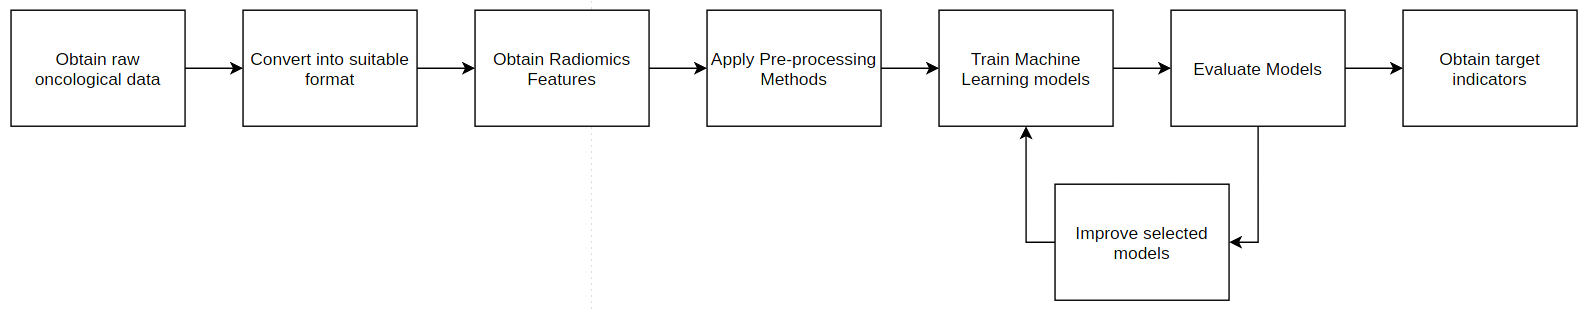
\includegraphics[width=6in]{img1.png}
\caption{Project Pipeline}
\label{img1}
\end{figure*}

\subsection{Obtaining Raw data}

In order to obtain distinct yet comparable subjects, a cohort dataset of 89 patients was selected in this study. The dataset consisted of four intrinsic molecular subtypes of breast cancer which are contrasted on the genes a cancerous cell expresses. The dataset has been descibed in Table $\ref{tb1}$.

\begin{table*}[!b]
\centering
\caption{Data Description}
\label{tb1}
\begin{tabular}{| c | c | c | c | c | c |}
\hline
Subtype & Number of paitents & Estrogen Receptor & Progesterone Receptor & HER2 & KI67 range\\
\hline
Luminal A & 29 & + & +/- & - & [5,20] \\
Luminal B & 36 & + & +/- & +/- & [25,80] \\
Triple Negative(TN) & 19 & - & - & - & [20,90] \\
HER & 5 & - & - & + & [30,50]\\
\hline
\end{tabular}
\end{table*}

For each of the patient, a CT scan was conducted to obtain cross-sectional images of the hypothesised tumor location. CT scans provide a more detailed description of the patients condition by increasing the radiation level the patient is exposed to. Once the scan is completed three views are obtained namely, Axial, Sagittal and Coronal. DICOM (Digital Imaging and Communication in Medicine) images were obtained after the scan. For each patient 323 new studies were conducted with each study have 384 series which corresponded to 466 instances or images of the scan. Even though DICOM files are a standard format for medical imaging, NRRD (Nearly Raw Raster Data) files are anonymmized and contain no sensitive patient information. Moreover NRRD store the entire information in a single file as opposed to DICOM imaging.

% \begin{figure*}[!b]
% \centering
% 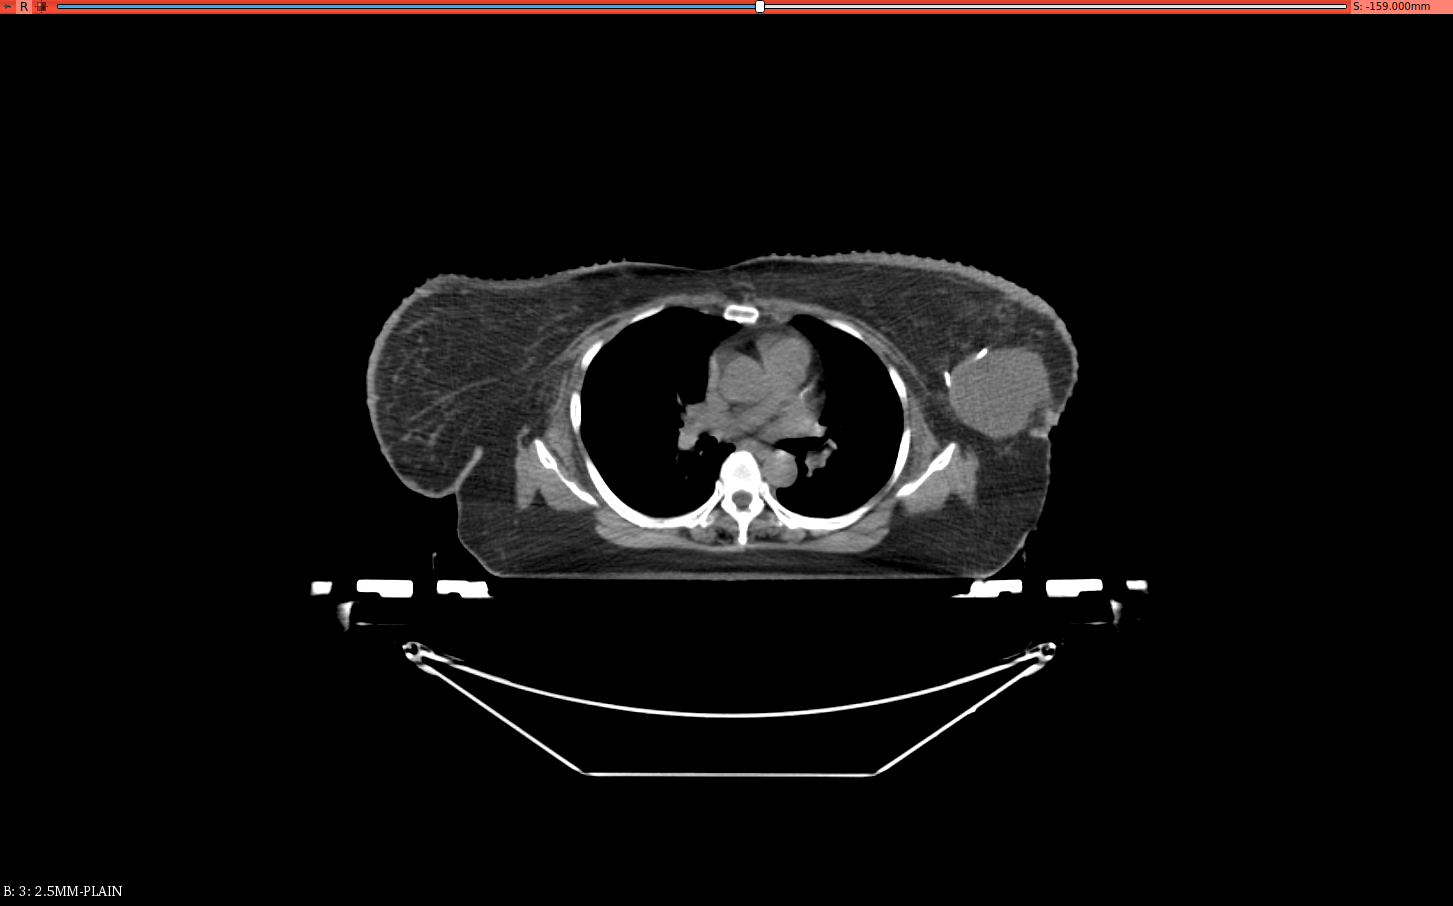
\includegraphics[width=4in]{img2.png}
% \caption{Axial view with the tumor}
% \label{img2}
% \end{figure*}


\begin{figure*}[!b]
\centering
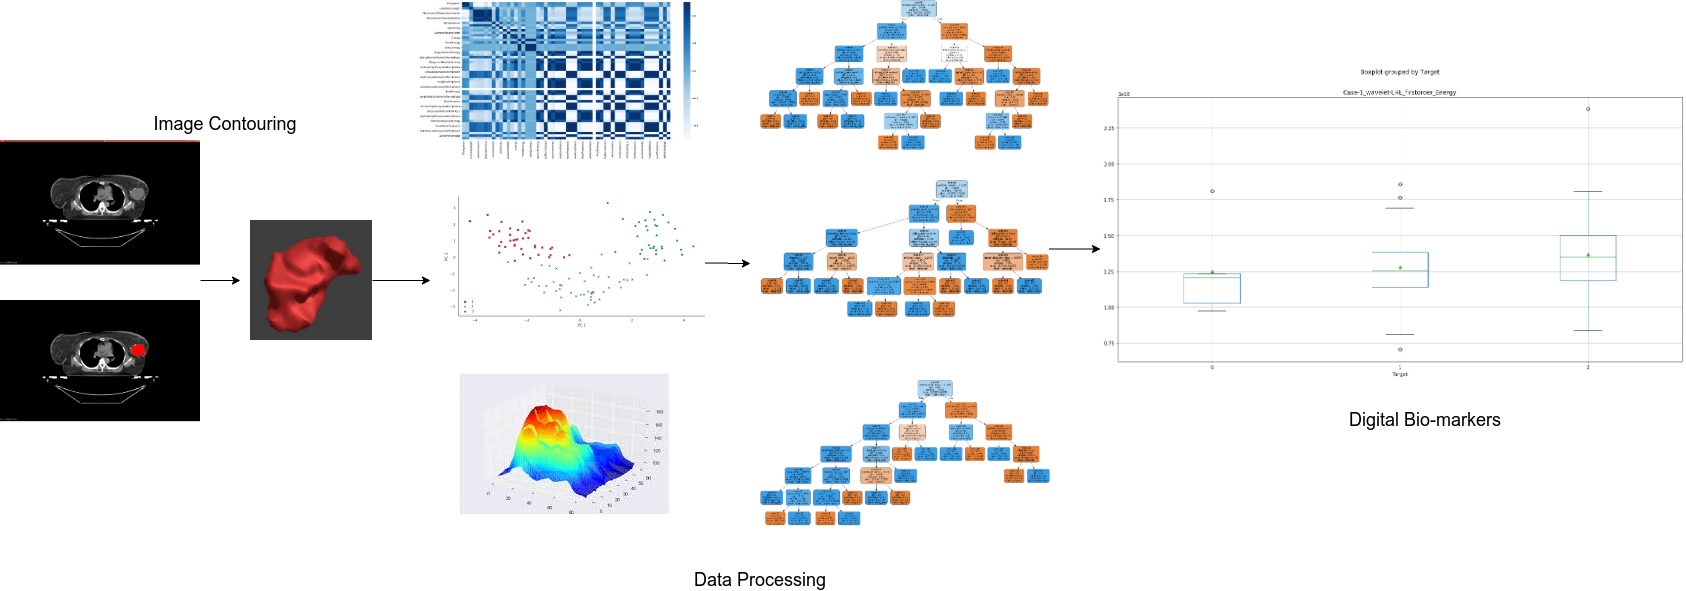
\includegraphics[width=7.5in]{im.png}
\caption{untitled}
\label{img2}
\end{figure*}

\subsection{Convert to a suitable format}

As mentioned previously, NRRD provides a more insightful appraoch to understanding medical imaging and recognizing inherent patterns in a concised format. The conversion was done with the help of the Plastimatch tool which is an open source software for image computation. Plastimatch takes the DICOM image which is described in a polyline vectorized format, and converts it into a series of pixels which is more prominently known as rasterization. The subroutine for rasterization of a DICOM image set with coordiantes $x$ and $y$ is shown below.

\begin{verbatim}
def rast(x, y, shape):
        nx, ny = draw.polygon(x, y, shape)
        nrrd = np.zeros(shape, dtype=np.bool)
        nrrd[ny, nx] = True 

        return nrrd
\end{verbatim}

Once this step is conducted, our image is in a compressed format, rife with information. Information extraction can be conducted through multiple means such as using neural networks, OCR recognition or pattern recognition algorithms. 

\subsection{Obtaining Radiomics Features}

Information extraction from images directly has certain drawbacks. For eg, consider tumor classification using a standard Convolutional Neural Network (CNN). The CNN might be extremely successful in determining the existense of a blob of mass and it's exact location. However diagnosing the exact nature and feature set of the tumor is extremely difficult for a CNN. This is because a CNN views the image as simply a collection of pixels without any regard to the information embedded in all the views of the data. 

To tackle this issue, we have utilized radiomics algorithms to extract feature sets from the medical images to reveal characteristics which are not captured by trained networks. The open-source Python library, PyRadiomics was used to mine out the required feature set. Before the actual extraction could be performed, a set of filters were applied on the NRRD to provide a comprehensive view of the data. The filters applied are listed in table $\ref{tb2}$. 

\begin{table*}[!b]
\centering
\caption{Applied Filters}
\label{tb2}
\begin{tabular}{| c | c | c |}
\hline
Filter & Description & Equation\\
\hline
Wavelet & Selective emphasizing or de-emphasizing of image in selected spatial frequency domain & -\\
(9)&&\\
\hline
Square & Square the image intensities & x := (cx)\textsuperscript{2}\\
\hline
Square Root & Compute root of image intensities & x := $\sqrt{cx}$\\
\hline
Laplacian of Gaussian & Applies a Laplacian of Gaussian filter to the input image  & $\frac{1}{(\sigma\sqrt{2\pi})\textsuperscript{3}}e\textsuperscript{-\sufr{x\textsuperscript{2}+y\textsuperscript{2}+z\textsuperscript{2}}{2\sigma\textsuperscript{2}}}$\\
$\sigma$ = 1, 2, 3&and yields a derived image for each sigma value specified&\\
\hline
Logarithm & Computes the natural logarithm of image intensities & c$\log(x+1)$\\
\hline
Exponential & Computes the exponential of the original image & e\textsuperscript{cx}\\
\hline
Gradient & Computes the gradient of the image & -\\
\hline
\end{tabular}
\end{table*}

PyRadiomics obtains radiomics features from the CT scan results in a stagewise manner. Initially the images are loaded into the platform by using SimpleITK which supports a gamut of image types along wit basic image processing techniques. In the next step, the filters descibed in $\ref{tb2}$ are applied using SimpleITK, PyWavelets, and Numpy. Finally, statistical and texture classes are used for feature extraction. The features so obtained, are stored in a dictionary format which suitable labels. 

To define a Region of Interest (ROI) and to check the dimensional constrainsts of the data, a mask file is utilized. The mask file contains the tumor's location demarcated by a radiologist. The features extracted are descibed by the Imaging Biomarker Standardization Initiative (IBSI) and have have been shown in tables $\ref{tb3}$ and $\ref{tb4}$.
% The mask image corresponding to Figure $\ref{img2}$ is shown in Figure $\ref{img3}$. Note the red mark demarcating the tumor is done by a radiologist as is standard procedure. The features are now extracted from the image set with the help of the mask file. 

% \begin{figure*}[!b]
% \centering
% 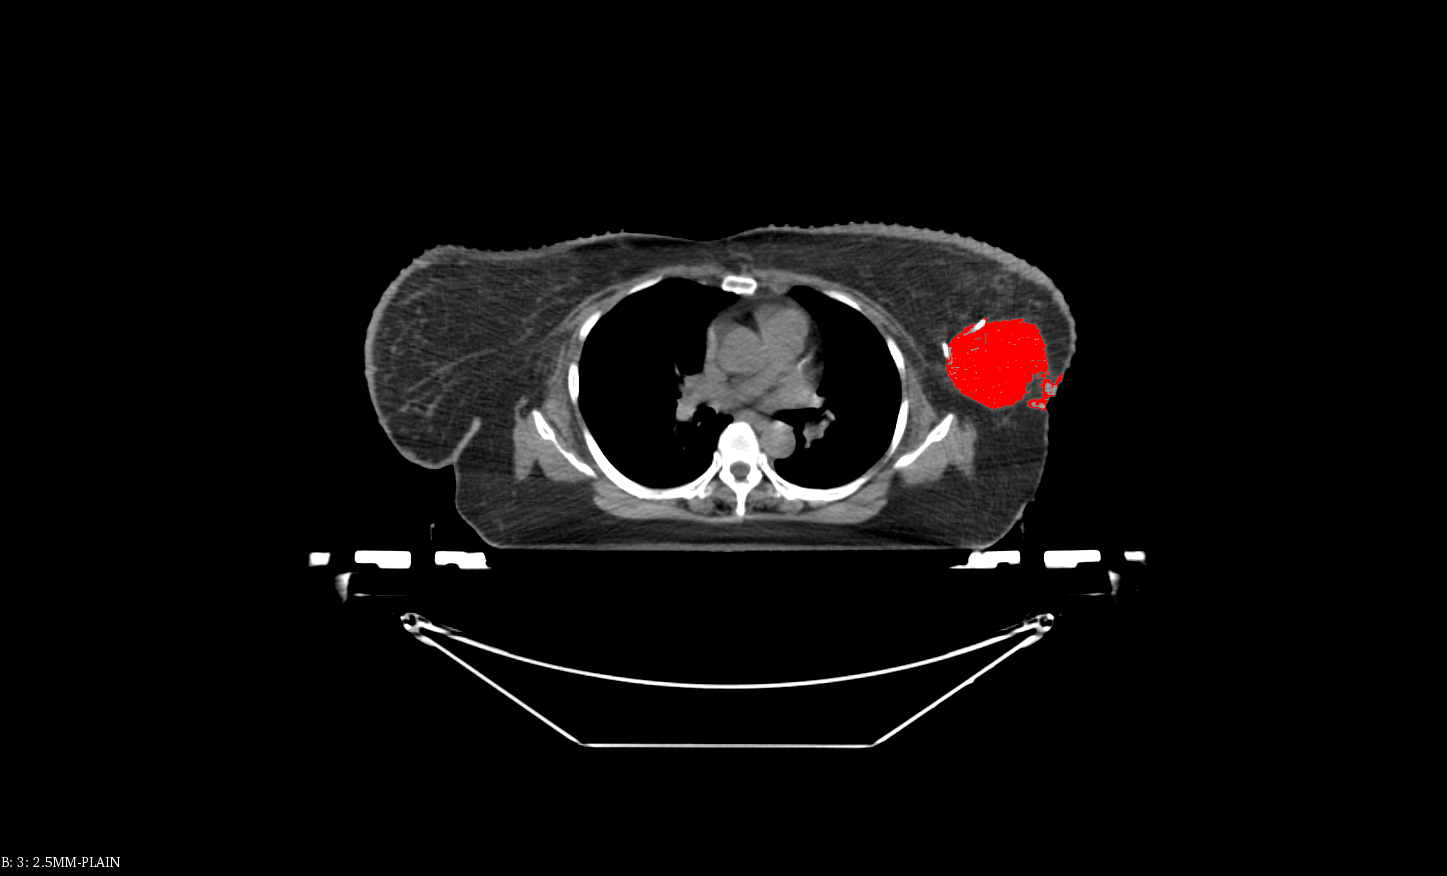
\includegraphics[width=4in]{img3.png}
% \caption{Mask image}
% \label{img3}
% \end{figure*}

\begin{table*}[!b]
\centering
\caption{Features-I}
\label{tb3}
\begin{tabular}{| c | c || c | c |}
\hline
Feature Class & Feature & Feature Class & Feature\\
\hline
& Elongation &&Autocorrelation\\
&Flatness&&Cluster\_Prominence\\
&Least\_Axis\_length&&Cluster\_Shade\\
&Major\_Axis\_Length&&Cluster\_Tendency\\
&Max\_2D\_Diameter\_Column&&Constrast\\
&Max\_2D\_Diameter\_Row&&Correlation\\
&Max\_2D\_Diameter\_Slice&&Difference\_Average\\
Shape&Max\_3D\_Diameter&&Difference\_Entropy\\
&Mesh\_Volume&&Difference\_Variance\\
&Minor\_Axis\_Length&&Inverse\_Variance\\
&Sphercity&&Joint\_Average\\
&Surface\_Area&Grey Level&Joint\_Energy\\
&Surface\_Volume&Co-occurance Matrix&Joint\_Entropy\\
&Voxel\_Volume&&MCC\\
&&&Maximum\_Probability\\
&&&Sum\_Average\\
&&&Sum\_Entropy\\
&&&Sum\_Squares\\
&&&Id\\
&&&Idm\\
&&&Idn\\
&&&Idmn\\
&&&Imc1\\
&&&Imc2\\
\hline
&10 Percentile&&Uniformity\\
&90 Percentile&&Normalized\_Uniformity\\
&Energy&&Variance\\
&Entropy&&High\_Run\_Emphasis\\
&Interquartile\_Range&&Long\_Run\_Emphasis\\
&Kurtosis&&Long\_High\_Run\_Emphasis\\
&Maximum&&Long\_Low\_Run\_Emphasis\\
&Mean\_Absolute\_Deviation&&Low\_Run\_Emphasis\\
First Order&Mean&Grey Level Run&Run\_Entropy\\
Statistics&Median&Length Matrix&Run\_Uniformity\\
&Minimum&&Run\_Uniformity\_Normalized\\
&Range&&Run\_Percentage\\
&Robust\_Mean\_Deviation&&Run\_Variance\\
&Robust\_Mean\_Squared&&Short\_Run\_Emphasis\\
&Skewness&&Short\_Run\_High\_Emphasis\\
&Total\_Energy&&Short\_Run\_Low\_Emphasis\\
&Uniformity&&\\
&Variance&&\\
\hline
\end{tabular}
\end{table*}

\begin{table*}[!b]
\centering
\caption{Features-II}
\label{tb4}
\begin{tabular}{| c | c |}
\hline
Feature Class & Feature\\
\hline
&Non\_Uniformity\\
&Non\_Uniformity\_Normalized\\
&Variance\\
&High\_Zone\_Emphasis\\
&Large\_Area\_Emphasis\\
&Large\_Area\_High\_Level\_Emphasis\\
&Large\_Area\_Low\_Level\_Emphasis\\
Grey Level Size&Low\_Zone\_Emphasis\\
Zone Matrix&Zone\_Non\_Uniformity\\
&Zone\_Non\_Uniformity\_Normalized\\
&Small\_Area\_Emphasis\\
&Small\_Area\_High\_Level\_Emphasis\\
&Small\_Area\_Low\_Level\_Emphasis\\
&Zone\_Entropy\\
&Zone\_Percentage\\
&Zone\_Variance\\
\hline
&Dependence\_Entropy\\
&Dependence\_Non\_Uniformity\\
&Dependence\_Non\_Uniformity\_Normalized\\
&Dependence\_Variance\\
&GL\_Non\_Uniformity\\
&GL\_Variance\\
Gray Level Size&High\_Emphasis\\
Zone Matrix&Large\_Dependence\_Emphasis\\
&Large\_Dependence\_High\_Emphasis\\
&Large\_Dependence\_Low\_Emphasis\\
&Low\_Emphasis\\
&Small\_Dependence\_Emphasis\\
&Small\_Dependence\_High\_Emphasis\\
&Small\_Dependence\_Low\_Emphasis\\
\hline
&Busyness\\
Neighbouring Gray Tone&Coarseness\\
Difference Matrix&Complexity\\
&Constrast\\
&Strength\\
\hline
\end{tabular}
\end{table*}

Therefore for each patient, the total number of features obtained are number of filters $\times$ number of features i.e, 17 $\times$ 100 = 1700 features. Once the entire feature set has been collected, the classification task can be started. 

\subsection{Applying Pre-processing Techniques}

From the 1700 features collected, not all of the features will contribute equally in the classification function. The process of preparing the input data for pattern learning by removing redundant characteristics, reducing noises and normalizing, selecting, and extracting features is termed as Data Pre-Processing. Multiple data pre-processing techniques have been applied to the feature set. These techniques have been descibed in Table $\ref{tb5}$.

\begin{table*}[!b]
\centering
\caption{Preprocessing techniques}
\label{tb5}
\begin{tabular}{| c | c |}
\hline
Method & Description\\
\hline
Missing Value Ratio & Removal of data columns where the ratio of missing values is greater than a set threshold \\
\hline
Low Varience Filter & Removal of normalized data columns where the variance is lesser than a set threshold\\
\hline
Highest correlation filter & Removal of data columns which are highly correlated leading to redundancy\\
\hline
Principle Component Analysis & Transformation of data to maximize variance under constraints\\
\hline
Fast Independent Component Analysis & Decomposition of signals to focus on mutual independence of data \\
\hline
Factor Analysis & Generating a common feature by reducing number of common variables \\
\hline
\end{tabular}
\end{table*}

Since the number of test subjects for each class is not similar, a threshold confidence level must be specified during the hypothesis testing phase. A 'P-value' is utilized in hypothesis testing to test the hypothesis under observation. A lower p-value corresponds to a higher confidence level in the predictions. The number of features selected after the pre-processing step is directly proportional to the p-value as a higher p-value will be more accomodating of even unimportant features. A grid for different p-values was created and the corresponding number of features were obtained.   

\subsection{Model-based Predictions}

Once the features have been narrowed down, we use a flavour of Ensemble Learning called SFORCE to classify test subjects into the predicted classes. SFORCE establishes a symbiotic relation between a predictive model (Random Forest) and an Ensemble model (AdaBoost). Both these models work on the presented data simlutaneously, aiding each other in the prediction process. Random Forests provides a strong learning system with the occasional pitfall of overfitting. The data is classified based the features which contrast the classes with the highest information content. The process of data classification using Random Forest is shown in Algorithm $\ref{alg:rf}$. AdaBoost solves the problem of overfitting by presenting the system with the misclassified data and forcing it to improve the overall performance. The two flavours of AdaBoost i.e, SAMME and SAMME.R have been descibed in Algorithms $\ref{alg:samme}$ and $\ref{alg:sammer}$. SFORCE combines the strength of Random Forests and takes care of the  drawbacks by using a Boosting algorithm to make the search process more concentrated as shown in Algorithm $\ref{alg:sforce}$. 

To obtain digital bio-markers, two cases studies were conducted from the avaiable cohort dataset. The first study involved classifying test subjects as TN or non TN subjects. In the second study, the Luminal-B dataset was set aside as the test dataset due to the close resemblance of it's characteristics with those of Luminal A. The model was trained to place the test subjects into the Luminal-A class with an accuracy of 72.7\%. The results for different p-values have been descibed in Tables $\ref{tb6}$ and $\ref{tb7}$. Based on these results,  box-plots have been obtained for the selected features which act as bio-markers for future reference.


\begin{table*}[!b]
\centering
\caption{TN vs Non-TN}
\label{tb6}
\begin{tabular}{| c | c | c | c |}
\hline
P-Value & Number of features & SAMME Accuracy & SAMME.R Accuracy\\
\hline
1&21&81.25&90.39\\
\hline
0.5&16&90.39&93.25\\
\hline
0.1&6&75&81.25\\
\hline
\end{tabular}
\end{table*}

\begin{table*}[!b]
\centering
\caption{HER vs Luminal-A vs TN}
\label{tb7}
\begin{tabular}{| c | c | c | c |}
\hline
P-Value & Number of features & SAMME Accuracy & SAMME.R Accuracy\\
\hline
1E-5&17&72&63.63\\
\hline
1E-6&15&70&72.7\\
\hline
17-5&13&72.7&70\\
\hline
\end{tabular}
\end{table*}

% \begin{algorithm}
% \begin{algorithmic}[1]
% \STATE Start
% \end{algorithmic}
% \end{algorithm}
\begin{algorithm}[!t]
\caption{: Ensemble Learning: Random Forest}\label{alg:rf}
\begin{algorithmic}[1]
\footnotesize
\STATE \textbf{// Input:} Data Set D = \{(\(x_1, y_1\)),(\(x_2, y_2\)), \dots\, ((\(x_m, y_m\))\}, Feature Set F, Randomization Factor R, Number of trees T 
\\\textbf{// Output:} Root node of i\textsuperscript{th} tree
\STATE - - - - - - - - - - - - - - - - - - - - - - - - - - - - - - - - - - - - - - - - - - - - -
\FOR { $ \forall i \in \{1, 2, \dots\, T\}$ } 
\STATE {$ N_i \gets$ Root node of i\textsuperscript{th} tree}
\IF {All targets belong to same class i.e $ y_i $ or $F \in \emptyset $ }
\STATE { Return $N_i$}
\ENDIF
%\If {$F \in \emptyset $} \STATE { Return $N_i$} \ENDIF
\STATE { $ D_i \leftarrow $ bootstraped sample from D }  
\FOR {Each node}
\STATE { $ f \leftarrow $ Randomly selected $ R $ features from $ F $ }
\STATE { $ N_f \leftarrow $ Best Feature from $ f $ features }
\STATE { $ N_p \leftarrow $ Best Split based on $ N_f $ }
\ENDFOR
\ENDFOR
\STATE { \textbf{ return $ N_i $ } }
\end{algorithmic}
\end{algorithm}

\begin{algorithm}[!t]
\caption{: Stagewise Additive Modeling: SAMME }\label{alg:samme}
\begin{algorithmic}[1]
\footnotesize
%\\\textbf{// Purpose:} Pairwise Sequence Alignment of query sequences and reference index elements with DP algorithms
\STATE \textbf{// Input:} Data Set D = \{(\(x_1, y_1\)),(\(x_2, y_2\)), \dots\, ((\(x_m, y_m\))\}, Number of Learning Rounds T, Learning Algorithm $ \epsilon $  
\STATE \textbf{// Output:} sign($\sum_{t=1}^{T} \alpha_t.C_t$)
\STATE - - - - - - - - - - - - - - - - - - - - - - - - - - - - - - - - - - - - - - - - - - - - -
\STATE \emph{$D_1$(x)} = 1/m \COMMENT{Initialize the weight distribution}
\FOR { $ t = \{1, 2, \dots\, T\}$ } 
\STATE \emph{$C_t$} = $\epsilon$(D,\emph{$D_t$}) \COMMENT{Create classifier $C_t$}
\STATE $e_t$ = \emph{$P_{x \sim \emph{D}}$}(\emph{$h_t$(x) $\neq$ f(x)}) \COMMENT{Calculate error $e_t$}
\STATE $\alpha_t$ = $log{\dfrac{1-e_t}{e_t}}$ + log($\emph{K-1}$) \COMMENT{Calculate the weight $h_t$}
\STATE \emph{$D_i$(x)} $\leftarrow$ \emph{$D_i$(x)}.exp($\alpha_t$.P($\emph{$C_i$} \neq f(x)$)) \COMMENT{Update the distribution $D_t$}, $ i = \{1, 2, \dots\, m\}$
\STATE {Renormalize \emph{$D_t$(x)}}
\ENDFOR 
\end{algorithmic}
\end{algorithm}

\begin{algorithm}[!t]
\caption{: Stagewise Additive Modeling for Real Value Predictions: SAMME.R }\label{alg:sammer}
\begin{algorithmic}[1]
\footnotesize
%\\\textbf{// Purpose:} Pairwise Sequence Alignment of query sequences and reference index elements with DP algorithms
\STATE \textbf{// Input:} Data Set D = \{(\(x_1, y_1\)),(\(x_2, y_2\)), \dots\, ((\(x_m, y_m\))\}, Number of Learning Rounds T, Learning Algorithm $ \epsilon $  
\STATE \textbf{// Output:} sign($\sum_{t=1}^{T} \alpha_t.C_t$)
\STATE - - - - - - - - - - - - - - - - - - - - - - - - - - - - - - - - - - - - - - - - - - - - -
\STATE \emph{$D_1$(x)} = 1/m \COMMENT{Initialize the weight distribution}
\FOR { $ t = \{1, 2, \dots\, T\}$ } 
\STATE \emph{$C_t$} = $\epsilon$(D,\emph{$D_t$}) \COMMENT{Create classifier $C_t$}
\STATE {$p_{kt}(x)$ = Prob($y=k|x$)}, $ k = \{1, 2, \dots\, K\}$
\STATE {$h_{kt}(x)$} $\leftarrow$ ($K$ - 1)($log{p_{kt}(x)}$ - $\dfrac{1}{K}.\sum_{k'} log{p_{k't}}$(x))
%\STATE $e_t$ = \emph{$P_{x~\emph{D}}$}(\emph{$h_t$(x) $\neq$ f(x)}) \COMMENT{Calculate error $e_t$}
%\STATE $\alpha_t$ = $log{\dfrac{1-e_t}{e_t}}$ + log($\emph{K-1}$) \COMMENT{Calculate the weight $h_t$}
\STATE \emph{$D_i$(x)} $\leftarrow$ \emph{$D_i$(x)}.exp($\dfrac{1-K}{K}$.$y_{i}^{ \textbf{T} }.log({p_t}(x_i)$)    ) \COMMENT{Update the distribution $D_t$, $ i = \{1, 2, \dots\, m\}$ }
\STATE {Renormalize \emph{$D_t$(x)}}
\ENDFOR 
\end{algorithmic}
\end{algorithm}

\begin{algorithm}[!t]
\caption{: Ensemble of Ensemble: SFORCE}\label{alg:sforce}
\begin{algorithmic}[1]
\footnotesize
%\\\textbf{// Purpose:} Pairwise Sequence Alignment of query sequences and reference index elements with DP algorithms
\STATE \textbf{// Input:} Data Set D = \{(\(x_1, y_1\)),(\(x_2, y_2\)), \dots\, ((\(x_m, y_m\))\}, Feature Set F, Randomization Factor R, Number of trees T,Number of Learning Rounds T', Learning Algorithm $ \epsilon $   
\STATE \textbf{// Output:} Root node of i\textsuperscript{th} Boosted Tree
\STATE - - - - - - - - - - - - - - - - - - - - - - - - - - - - - - - - - - - - - - - - - - - - -
\STATE{Random Forest}
\FOR { $ \forall i \in \{1, 2, \dots\, T\}$ } 
\STATE {$ N_i \gets$ Root node of i\textsuperscript{th} tree}
\IF {All targets belong to same class i.e $ y_i $ or $F \in \emptyset $ } 
\STATE Call SAMME.R with {$N_i$} 
\ENDIF
%\If {$F \in \emptyset $} \STATE { Return $N_i$} \ENDIF
\STATE { $ D^i \leftarrow $ bootstraped sample from D }  
\FOR {Each node}
\STATE { $ f \leftarrow $ Randomly selected $ R $ features from $ F $ }
\STATE { $ N_f \leftarrow $ Best Feature from $ f $ features }
\STATE { $ N_p \leftarrow $ Best Split based on $ N_f $ }
\STATE Call SAMME.R with {$N_i$}
\ENDFOR
\ENDFOR
\STATE { \textbf{ return $ N_i $ } }
\STATE - - - - - - - - - - - - - - - - - - - - - - - - - - - - - - - - - - - - - - - - - - - - -
\STATE{SAMME/SAMME.R}
\STATE \emph{$D_1$(x)} = 1/m \COMMENT{Initialize the weight distribution}
\FOR { $ t = \{1, 2, \dots\, T\}$ } 
\STATE \emph{$C_t$} = $\epsilon$(D,\emph{$D_t$}) \COMMENT{Create classifier $C_t$}
\STATE {$p_{kt}(x)$ = Prob($y=k|x$)}, $ k = \{1, 2, \dots\, K\}$
\STATE {$h_{kt}(x)$} $\leftarrow$ ($K$ - 1)($log{p_{kt}(x)}$ - $\dfrac{1}{K}.\sum_{k'} log{p_{k't}}$(x))
%\STATE $e_t$ = \emph{$P_{x~\emph{D}}$}(\emph{$h_t$(x) $\neq$ f(x)}) \COMMENT{Calculate error $e_t$}
%\STATE $\alpha_t$ = $log{\dfrac{1-e_t}{e_t}}$ + log($\emph{K-1}$) \COMMENT{Calculate the weight $h_t$}
\STATE \emph{$D_i$(x)} $\leftarrow$ \emph{$D_i$(x)}.exp($\dfrac{1-K}{K}$.$y_{i}^{ \textbf{T} } .log({p_t}(x_i)$)    ) \COMMENT{$ i = \{1, 2, \dots\, m\}$}
\STATE {Renormalize \emph{$D_t$(x)}}
\STATE Call Random Forest with {($\sum_{t=1}^{T'} \alpha_t.C_t$)}
\ENDFOR
\end{algorithmic}
\end{algorithm}

\begin{algorithm}[!t]
\caption{untitled}\label{main}
\begin{algorithmic}[1]
\footnotesize
\STATE //Input Image dataset $D\textsubscript{n}$ and masks $D\textsubscript{m}$ 
\STATE //Output Predicted Class
\FOR {Each image $i$ in $D\textsubscript{n}$}
\STATE Convert image to a suitable format using conversion software
\STATE Call the pre-processsing techniques on the formatted images
\STATE Using mask $j$ for corresponding $i$, extract radiomics features
\STATE Create a grid of p-values
\FOR {EACH value in grid}
\STATE Call Algorithm $\ref{alg:sforce}$ with related feature set
\ENDFOR
\STATE Obtain accuracy levels and digital bio-markers
\ENDFOR
\end{algorithmic}
\end{algorithm}
% Computer Society journal (but not conference!) papers do something unusual
% with the very first section heading (almost always called "Introduction").
% They place it ABOVE the main text! IEEEtran.cls does not automatically do
% this for you, but you can achieve this effect with the provided
% \IEEEraisesectionheading{} command. Note the need to keep any \label that
% is to refer to the section immediately after \section in the above as
% \IEEEraisesectionheading puts \section within a raised box.




% The very first letter is a 2 line initial drop letter followed
% by the rest of the first word in caps (small caps for compsoc).
% 
% form to use if the first word consists of a single letter:
% \IEEEPARstart{A}{demo} file is ....
% 
% form to use if you need the single drop letter followed by
% normal text (unknown if ever used by the IEEE):
% \IEEEPARstart{A}{}demo file is ....
% 
% Some journals put the first two words in caps:
% \IEEEPARstart{T}{his demo} file is ....
% 
% Here we have the typical use of a "T" for an initial drop letter
% and "HIS" in caps to complete the first word.
% \IEEEPARstart{T}{his} demo file is intended to serve as a ``starter file''
% for IEEE Computer Society journal papers produced under \LaTeX\ using
% IEEEtran.cls version 1.8b and later.
% % You must have at least 2 lines in the paragraph with the drop letter
% % (should never be an issue)
% I wish you the best of success.
% 
% \hfill mds
%  
% \hfill August 26, 2015
% 
% \subsection{Subsection Heading Here}
% Subsection text here.
% 
% % needed in second column of first page if using \IEEEpubid
% %\IEEEpubidadjcol
% 
% \subsubsection{Subsubsection Heading Here}
% Subsubsection text here.


% An example of a floating figure using the graphicx package.
% Note that \label must occur AFTER (or within) \caption.
% For figures, \caption should occur after the \includegraphics.
% Note that IEEEtran v1.7 and later has special internal code that
% is designed to preserve the operation of \label within \caption
% even when the captionsoff option is in effect. However, because
% of issues like this, it may be the safest practice to put all your
% \label just after \caption rather than within \caption{}.
%
% Reminder: the "draftcls" or "draftclsnofoot", not "draft", class
% option should be used if it is desired that the figures are to be
% displayed while in draft mode.
%
%\begin{figure}[!t]
%\centering
%\includegraphics[width=2.5in]{myfigure}
% where an .eps filename suffix will be assumed under latex, 
% and a .pdf suffix will be assumed for pdflatex; or what has been declared
% via \DeclareGraphicsExtensions.
%\caption{Simulation results for the network.}
%\label{fig_sim}
%\end{figure}

% Note that the IEEE typically puts floats only at the top, even when this
% results in a large percentage of a column being occupied by floats.
% However, the Computer Society has been known to put floats at the bottom.


% An example of a double column floating figure using two subfigures.
% (The subfig.sty package must be loaded for this to work.)
% The subfigure \label commands are set within each subfloat command,
% and the \label for the overall figure must come after \caption.
% \hfil is used as a separator to get equal spacing.
% Watch out that the combined width of all the subfigures on a 
% line do not exceed the text width or a line break will occur.
%
%\begin{figure*}[!t]
%\centering
%\subfloat[Case I]{\includegraphics[width=2.5in]{box}%
%\label{fig_first_case}}
%\hfil
%\subfloat[Case II]{\includegraphics[width=2.5in]{box}%
%\label{fig_second_case}}
%\caption{Simulation results for the network.}
%\label{fig_sim}
%\end{figure*}
%
% Note that often IEEE papers with subfigures do not employ subfigure
% captions (using the optional argument to \subfloat[]), but instead will
% reference/describe all of them (a), (b), etc., within the main caption.
% Be aware that for subfig.sty to generate the (a), (b), etc., subfigure
% labels, the optional argument to \subfloat must be present. If a
% subcaption is not desired, just leave its contents blank,
% e.g., \subfloat[].


% An example of a floating table. Note that, for IEEE style tables, the
% \caption command should come BEFORE the table and, given that table
% captions serve much like titles, are usually capitalized except for words
% such as a, an, and, as, at, but, by, for, in, nor, of, on, or, the, to
% and up, which are usually not capitalized unless they are the first or
% last word of the caption. Table text will default to \footnotesize as
% the IEEE normally uses this smaller font for tables.
% The \label must come after \caption as always.
%



% Note that the IEEE does not put floats in the very first column
% - or typically anywhere on the first page for that matter. Also,
% in-text middle ("here") positioning is typically not used, but it
% is allowed and encouraged for Computer Society conferences (but
% not Computer Society journals). Most IEEE journals/conferences use
% top floats exclusively. 
% Note that, LaTeX2e, unlike IEEE journals/conferences, places
% footnotes above bottom floats. This can be corrected via the
% \fnbelowfloat command of the stfloats package.
% 
% 
% 
% 
% \section{Conclusion}
% The conclusion goes here.





% if have a single appendix:
%\appendix[Proof of the Zonklar Equations]
% or
%\appendix  % for no appendix heading
% do not use \section anymore after \appendix, only \section*
% is possibly needed

% use appendices with more than one appendix
% then use \section to start each appendix
% you must declare a \section before using any
% \subsection or using \label (\appendices by itself
% starts a section numbered zero.)
%


% \appendices
% \section{Proof of the First Zonklar Equation}
% Appendix one text goes here.
% 
% % you can choose not to have a title for an appendix
% % if you want by leaving the argument blank
% \section{}
% Appendix two text goes here.
% 
% 
% % use section* for acknowledgment
% \ifCLASSOPTIONcompsoc
%   % The Computer Society usually uses the plural form
%   \section*{Acknowledgments}
% \else
%   % regular IEEE prefers the singular form
%   \section*{Acknowledgment}
% \fi
% 
% 
% The authors would like to thank...


% Can use something like this to put references on a page
% by themselves when using endfloat and the captionsoff option.
\ifCLASSOPTIONcaptionsoff
  \newpage
\fi



% trigger a \newpage just before the given reference
% number - used to balance the columns on the last page
% adjust value as needed - may need to be readjusted if
% the document is modified later
%\IEEEtriggeratref{8}
% The "triggered" command can be changed if desired:
%\IEEEtriggercmd{\enlargethispage{-5in}}

% references section

% can use a bibliography generated by BibTeX as a .bbl file
% BibTeX documentation can be easily obtained at:
% http://mirror.ctan.org/biblio/bibtex/contrib/doc/
% The IEEEtran BibTeX style support page is at:
% http://www.michaelshell.org/tex/ieeetran/bibtex/
%\bibliographystyle{IEEEtran}
% argument is your BibTeX string definitions and bibliography database(s)
%\bibliography{IEEEabrv,../bib/paper}
%
% <OR> manually copy in the resultant .bbl file
% set second argument of \begin to the number of references
% (used to reserve space for the reference number labels box)
\begin{thebibliography}{1}

\bibitem{IEEEhowto:kopka}
H.~Kopka and P.~W. Daly, \emph{A Guide to \LaTeX}, 3rd~ed.\hskip 1em plus
  0.5em minus 0.4em\relax Harlow, England: Addison-Wesley, 1999.

\end{thebibliography}

% biography section
% 
% If you have an EPS/PDF photo (graphicx package needed) extra braces are
% needed around the contents of the optional argument to biography to prevent
% the LaTeX parser from getting confused when it sees the complicated
% \includegraphics command within an optional argument. (You could create
% your own custom macro containing the \includegraphics command to make things
% simpler here.)
%\begin{IEEEbiography}[{\includegraphics[width=1in,height=1.25in,clip,keepaspectratio]{mshell}}]{Michael Shell}
% or if you just want to reserve a space for a photo:
% 
% \begin{IEEEbiography}{Michael Shell}
% Biography text here.
% \end{IEEEbiography}
% 
% % if you will not have a photo at all:
% \begin{IEEEbiographynophoto}{John Doe}
% Biography text here.
% \end{IEEEbiographynophoto}
% 
% % insert where needed to balance the two columns on the last page with
% % biographies
% %\newpage
% 
% \begin{IEEEbiographynophoto}{Jane Doe}
% Biography text here.
% \end{IEEEbiographynophoto}

% You can push biographies down or up by placing
% a \vfill before or after them. The appropriate
% use of \vfill depends on what kind of text is
% on the last page and whether or not the columns
% are being equalized.

%\vfill

% Can be used to pull up biographies so that the bottom of the last one
% is flush with the other column.
%\enlargethispage{-5in}



% that's all folks
\end{document}


